% 4-7. előadás

\chapter{Szuperskalár architektúrák (párhuzamos kibocsátás)}

\section{Bevezetés}
A futószalag architektúrájú processzorok óraciklusonként csak egy kimenetet tudtak előállítani, ami korlátozta a teljes CPU sebességét.
Erre jelent megoldást a szuperskalár architektúra (1990 környékén jelent meg), aminek alkalmazásával elérhető a párhuzamos kibocsátás.
A szuperskalár architectúrákat első, második és harmadik generációra oszthatjuk.
A második és harmadik generációban már multimédiás (utasításon belüli párhuzamosság) képességek is megjelentek.

\section{Közös jellemzőik}
\begin{itemize}
    \item A dekódoló egységből képes óraciklusonként több utasítást kibocsátani (ennek száma a kibocsátási ráta, első generációnál 2-3, másodiknál 4-6).
    \item Időbeli és térbeli párhuzamosság (több futószalag párhuzamosan).
    \item Maguk küzdenek meg a függőségekkel (dinamikusan, extra hardverek segítségével, pl. adattípusonként külön regisztertár).
    \item Kompatibilitás: evolúció, azaz kompatibilis marad a korábbi futószalag architektúrákkal. Így a régi programok is futhatnak rajta.
\end{itemize}

\section{Harvard architektúra}
1944-ben írták le, lényege, hogy az adat és a programkód fizikailag elkülönített útvonalakon mozog.
Következménye, hogy párhuzamos adatutak jönnek létre, így növekszik a teljesítmény.
A szuperskalár architektúrák az L1 cache-nél alkalmaznak egy módosított Harvard architektúrát, ahol az utasítás és az adat külön tárolódik.
Az egyik eltérés az eredeti Harvard architektúrától, hogy képes programkódot is adatként betölteni.
Az L2 és L3 gyorsítótárakban megosztott tárhely van az adatok és utasítások részére.
Ezekből is látható, hogy a mai processzorok tervezésénél felhasználják mind a Harvard, mint a Neumann elveket.

\subsection{Vezérlési vázlat}
A Neumann elvű processzoroknál egy óraciklus alatt vagy adat, vagy utasítás lehívása történhetett meg.
A Harvard architektúráknál ezzel szemben egy vezérlőegység (CONTROL) hívja le az utasítást az instruction cache-ből (INSTR adatút), majd ez alapján jelet küld a data cache-nek, hogy az ALU-ba milyen címen lévő adat kerüljön (CONTROL\&ADDR).
Ezzel egyidőben az instruction cache felé is küld CONTROL\&ADDR jelet, tehát a következő órajelre az adat és a következő utasítás egyszerre hívódik le.
A CONTROL egység felel az ALU irányításáért is, az ALU az IN és OUT adatutakon kommunikálhat a perifériákkal, a STATUS adatúton pedig visszacsatolást biztosít a vezérlőegység számára.
Az egész működést a CLOCK által kibocsátott órajel irányítja.
Ennek a vázlata látható a \ref{fig:harvard}. ábrán.
Ezt a felépítést használják a modern processzorok is.
\begin{figure}[h]
    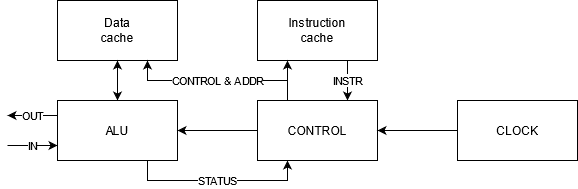
\includegraphics[width=0.6\textwidth]{harvard}
    \centering
    \caption{Harvard architektúra vezérlési vázlata}
    \label{fig:harvard}
\end{figure}

\subsection{Előnyei}
\begin{itemize}
    \item Képes párhuzamosan adatot és utasítást olvasni, vagy írni cache nélkül is.
    \item Az adat és utasítás tárolók különálló címtartománnyal rendelkeznek, amikben a címek különböző hosszúak is lehetnek (pl. utasítás címek 32 bit, adat címek 64 bit).
\end{itemize}

\section{Első generációs szuperskalárok (keskeny szuperskalárok)}

\subsection{Jellemzői}
\begin{itemize}
    \item Közvetlen, vagyis nem pufferelt kibocsátás: a CPU a dekódolt utasítást közvetlenül küldi a végrehajtó egységhez.
    \item Statikus elágazásbecslés. Az egyik ilyen megoldás a fix (mindig ugrik) elágazásbecslés, a másik lehetőség a programkód bizonyos tulajdonságai alapján létrehozott statikus elágazásbecslés. A statikus elágazásbecslést a fetch alrendszer végzi, így nincs ugrási buborék.
    \item Gyorsítótár a memória lassúságának kiküszöbölésére, itt már megjelentek a kétszintű gyorsítótárak is: L1 cache a processzorlapkán, L2 különálló lapkán.
    \item Különálló adat és utasítás az első szintű gyorsítótárban (ütközik a Neumann elvekkel, mivel az utasítás és az adat külön operatív tárban tárolódik $\rightarrow$ Harvard architektúra).
    \item Az operatív tár és az L2 cache közös az adat és utasítás számára $\rightarrow$ Neumann architektúra.
    \item Az előző két pontból következik, hogy az L1 cache elérése során Harvard elvűként, a memória és az L2 cache elérésekor pedig Neumann elvűként működik a processzor. Ezt a megoldást használják ma is, pl. az x86-os architektúra.
\end{itemize}

\subsection{Utasításablak}
Az utasításablak egy olyan puffer, amely az óraciklusonként kibocsátott utasításokat tartalmazza (\ref{fig:utasitasablak}. ábra).
Az utasításablak pufferből kerül feltöltésre, utasítás kibocsátáskor kiürül. Itt történik a dekódolás és a függőség ellenőrzés.
A végrehajtható utasítások kibocsátásra kerülnek, tehát közvetlenül a végrehajtó egységbe kerülnek.
A végrehajtható utasítás olyan utasítás, aminek nincs függősége.
A függőséggel rendelkező utasítások addig maradnak az utasításablakban, amíg a függőség meg nem szűnik.
\begin{figure}[H]
    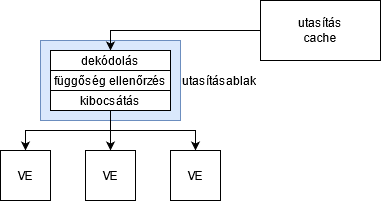
\includegraphics[width=0.6\textwidth]{utasitasablak}
    \centering
    \caption{Az utasításablak működése}
    \label{fig:utasitasablak}
\end{figure}
\paragraph{Utasítás pótlásának módjai:}
\begin{itemize}
    \item A kibocsátott utasításokat egyenként pótoljuk.
    \item A kibocsátott utasításokat egyszerre pótoljuk (megvárjuk, hogy az összes utasítás kiürüljön).
\end{itemize}
\paragraph{Utasítás végrehajtás és kibocsátás módjai:}
\begin{itemize}
    \item sorrendben
    \item sorrenden kívül
\end{itemize}
\paragraph{Alkalmazása szuperskalár processzorokban:} az első generációs szuperskalár architektúrák az utasításablakot egyszerre töltötték fel és sorrendi utasítás kibocsátást alkalmaztak.
A sorrendi kibocsátás hátránya, hogy egy függő utasítás a függőség megszűnéséig blokkolja a kibocsátást, így a végrehajtó egységek kihasználatlanul álltak.
Ez volt az első generációs szuperskalárok legnagyobb problémája.
\paragraph{Példa egyszerre pótló és sorrendben kibocsátó utasításablakra:} 3 végrehajtó egységünk van, az utasításablak kezdeti tartalma pedig két független és egy függőséggel rendelkező utasítás.
Jelöljük körrel a független utasításokat és teli körrel a függő utasításokat. Az adott óraciklusban kibocsátott utasításokat jobbra mutató nyíl jelzi.
Az utasításablak tartalma a \ref{fig:utasitasablak_pelda1}. ábrán látható.
Az első óraciklusban (C\textsubscript{i}) az I\textsubscript{2} utasításnak függősége van, így még nem bocsátható ki, a sorrendiség miatt pedig I\textsubscript{3} sem.
I\textsubscript{2} és I\textsubscript{3} a második óraciklusban (C\textsubscript{i+1}) kerül kibocsátásra.
Ezután új utasításokat hívunk le (I\textsubscript{4}, I\textsubscript{5} és I\textsubscript{6}).
I\textsubscript{4}-et és I\textsubscript{5}-öt rögtön ki is tudjuk bocsátani, mivel nincs függőségük, és a sorrendiség miatt I\textsubscript{6} függősége se akadályozza őket.
I\textsubscript{6} függőségének feloldására viszont két óraciklust kell várnunk, ezért csak a C\textsubscript{i+5} óraciklusban bocsátható ki.
Mivel megint kiürült az utasításablak, újabb három utasítást hívunk le.
Ebben az óraciklusban viszont egyetlen utasítást se tudunk kibocsátani, mivel a sorrendiség miatt I\textsubscript{7} függősége I\textsubscript{8}-at és I\textsubscript{9}-et is akadályozza.
Ezen utasítások kibocsátása csak a C\textsubscript{i+6} óraciklusban lehetséges.
\begin{figure}[h]
    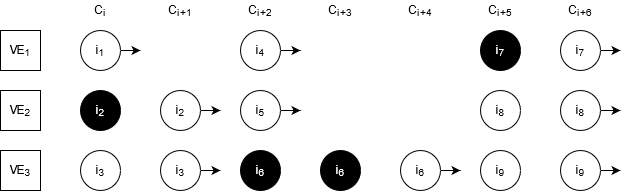
\includegraphics[width=0.8\textwidth]{utasitasablak_pelda1}
    \centering
    \caption{Az utasításablak tartalma egyszerre történő feltöltés és sorrendbeli kibocsátás esetés}
    \label{fig:utasitasablak_pelda1}
\end{figure}
\paragraph{Egyszerre pótló és sorrendben kibocsátó utasításablak értékelése:} a tapasztalat azt mutatja, hogy az ilyen elven működő processzor kibocsátási rátája közelít az 1 utasítás/ciklushoz.
Tehát a jóval több tranzisztor és bonyolultabb felépítés ellenére nem sokkal gyorsabb, mint a futószalag processzorok.
A keskeny szuperskalár név innen ered.

\subsection{Végrehajtási modell RISC architektúrák esetén}
A teljes rendszer feldolgozási sebességét az alrendszerek átbocsátási képessége határozza meg.
Az alrendszerek jellege és száma az adott mikroaarchitektúrától függ.
A végrehajtási modell három részből áll:
\begin{itemize}
    \item első rész: feladatai az utasítás lehívás és az utasításablak feltöltése
    \item utasításablak
    \item hátsó rész: feladata az utasításablak kiürítése (dekódolás, függőség ellenőrzés, kibocsátás), végrehajtás és a visszaírás.
\end{itemize}
Ennek az egyszerűsített modellje látható a \ref{fig:risc_vegrehajtas}. ábrán.
Mivel az ábra RISC architektúrát mutat be, az adat cache közvetlenül nem érhető el, csak a regisztertár.
A regisztertár és az adat cache közötti adatmozgatást LOAD/STORE utasítások segítségével érhetjük el.
\begin{figure}[h]
    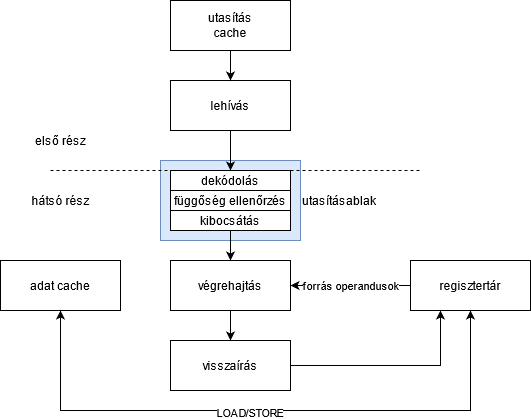
\includegraphics[width=0.6\textwidth]{risc_vegrehajtas}
    \centering
    \caption{Az első generációs szuperskalár RISC architektúrák végrehajtási modellje}
    \label{fig:risc_vegrehajtas}
\end{figure}
\paragraph{Szélesség:} az alrendszerek átbocsátási képességét nevezzük szélességnek.
A teljes rendszer szélességét a legkeskenyebb alrendszer szélessége határozza meg.

\subsection{Szűk keresztmetszetek}
Az első generációs szuperskalároknál a következő szűk keresztmetszetek lépnek fel:
\begin{itemize}
    \item kibocsátás,
    \item memória,
    \item elágazásfeldolgozás és
    \item függőségek.
\end{itemize}
A memória szűk keresztmetszetét cache bevezetésével, az elágazásét pedig statikus becsléssel csökkentették.
Nem tudták viszont kezelni a RAW függőségek és az adatfüggőségek által létrehozott szűk keresztmetszeteket.
Első generációs szuperskalároknál még az ál adatfüggőségek is blokkolnak.
A kibocsátási szűk keresztmetszet oka a közvetlen kibocsátás volt, így ezt se lehetett kezelni.
Következmény, hogy a végrehajtás általános célú alkalmazások esetén korlátozódik, és maximum 2 utasítás/ciklusra korlátozódik (RISC-nél max 3 utasítás/ciklus).
A gyakorlatban viszont még ezt se érte el, kb. 1 utasítás/ciklust eredményezett.

\subsection{Gyakorlati példa: Intel Pentium I}
A Pentium I-es CPU keskeny szuperskalár, CISC architektúrájú processzor volt.
Újdonság, hogy belül 64 bites, kívül pedig 32 bites buszokkal kapcsolódott (ez a megoldás nem egyedi, az Intel 8088 CPU kívül 8, belül 16 bites).
A nagyobb utasításokat így két óraciklusra tudta betölteni.
A processzor elvi működése a \ref{fig:pentium1}. ábrán látható.
\begin{figure}[h]
    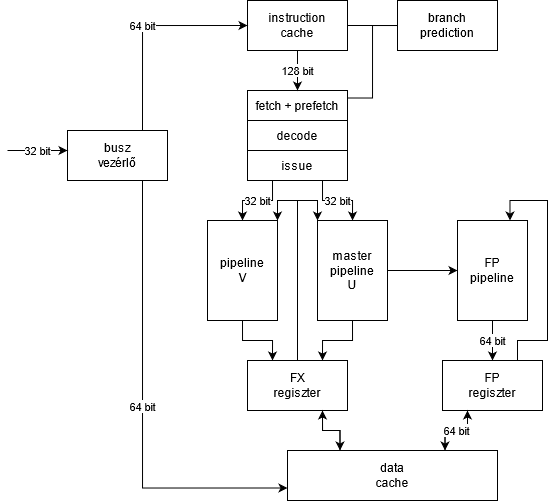
\includegraphics[width=0.8\textwidth]{pentium1}
    \centering
    \caption{Az Intel Pentium I processzor működése}
    \label{fig:pentium1}
\end{figure}
\paragraph{Futószalagok:}
2 futószalaggal rendelkezett, ebből egy dedikált (V) és egy univerzális (U vagy master).
A dedikált futószalag képes volt FX, L/S és Branch (elsősorban 1 ciklusos) utasítások végrehajtására, az univerzális pedig minden x86-os utasítást el tudott végezni (lebegőpontos számításokat is).
A két futószalag csak akkor dolgozott egyszerre, ha mindkettő egyszerű utasításokat dolgozott fel.
Mindkét futószalag 5 fokozatú volt (Fetch, Decode, Address Generation, Execute, Writeback).
Az U futószalag ezen kívül még 3 fokozatot tartalmazott, amit csak a lebegőpontos műveletekhez használt.
\paragraph{Ugrás előrejelzés:}
Újdonságnak számított még, hogy ugrás előrejelzést alkalmazott, ehhez 2 db prefetch buffert használt.
\paragraph{Cache:}
Az adat és az utasítás cache is 8 kbyte-os volt.

\section{Második generációs szuperskalárok}
Az első generációs szuperskalár CPU-k kibocsátási szűk keresztmetszete miatt az átbocsátóképesség növeléséhez át kellett tervezni az architektúrát.
Így születtek meg a második generációs szuperskalár processzorok.
Kibocsátási rátájuk kb. 4 utasítás/ciklus RISC és 3 utasítás/ciklus CISC architectúrák esetén, tehát az első generációhoz képest jelentős teljesítménynövekedés történt.

\subsection{Feltételei}
Egy CPU második generációs szuperskalárnak nevezhető, ha az alábbiak teljesülnek:
\begin{itemize}
    \item dinamikus utasítás ütemezés
    \item regiszter átnevezés
    \item elágazások előrejelzése dinamikus előrejelzéssel, ugrástörténet figyelembe vételével (ez kb. 90-95\%-os pontosságot biztosított)
    \item kifinomult és kibővített gyorsítótár alrendszer
    \item sorrenden kívüli kiküldés
\end{itemize}
A dinamikus utasítás átnevezés és a regiszter átnevezés segítségével sikerült kiküszöbölni a közvetlen kibocsátási szűk keresztmetszet.

\subsection{Példák}
\begin{itemize}
    \item Intel Pentium Pro
    \item AMD K6
    \item PowerPC 604
\end{itemize}

\subsection{Dinamikus elágazásbecslés}
Az elágazások történetét történet bitek formájában írja le. A dinamikus becslés lehet 1, 2 vagy 3 bites.
\paragraph{1 bites:} a történet bit értéke 0 vagy 1, attól függően, hogy ugrás vagy soros folytatás történt (a bitek jelentése architektúránként változik).
A következő elágazásnál a történet bit alapján döntötte el a CPU, hogy ugrás vagy soros végrehajtás következik.
\paragraph{2 bites:} a történet biteket 2 bittel ábrázoljuk. Az értékek a következők lehetnek:
\begin{itemize}
    \item 11 - határozott elágazás (mindenképp ugrik, általában ez a kezdeti állapot)
    \item 10 - gyenge elágazás
    \item 01 - gyenge soros folytatás
    \item 11 - határozott soros folytatás
\end{itemize}
Mivel legtöbbször az elágazásnál ugrás történik, ezért a történet bitek értéke kezdetben 11.
Amennyiben a következő elágazásnál mégis hibás volt az ugrás, a történeti bitek értéke 10-ra, gyenge elágazásra változik, tehát az ezt követő alkalommal megint meg fogja próbálni az ugrást.
Ha harmadszorra is hibás volt az ugrás, átkerül 01 állapotba, azaz gyenge soros folytatásra.

\subsection{Dinamikus utasítás ütemezés (várakoztatás, vagy pufferelt utasításkibocsátás)}
Lényege, hogy az utasítások kibocsátása pufferelt, sorrendi módon történik, a kiküldés viszont sorrenden kívüli.
Ez jelentősen megnöveli a mikroarchitektúra elejének átbocsátóképességét, valamint kiküszöböli a kibocsátási szűk keresztmetszetet.

\subsection{Sorrenden kívüli kiküldés}
A második generációs szuperskalároknál kibocsátáskor nincs függőségvizsgálat, ezért a lehívás, a dekódolás és a kibocsátás nominális rátával működhet, ami ebben az időben általában 3-4 utasítás/ciklus volt.
Az utasítások kibocsátáskor a kibocsátási pufferbe kerülnek, ez a várakoztató állomás.
A kibocsátási puffer lehet közös is, de előfordulhat, hogy a különböző típusú utasításoknak (FX, FP, stb.) külön pufferek vannak fenntartva.
A kibocsátási puffernek köszönhetően a vezérlő óraciklusonként akár több tucat utasítás közül is választhat, hogy mit küldjön ki végrehajtásra.
A döntés az állapot bitek alapján történik, a vezérlő ezek segítségével dönti el az utasításokról, hogy azok függők vagy függetlenek.
A CPU a független utasításokat küldi ki végrehajtásra.
Ez a működés látható a \ref{fig:kikuldes}. ábrán.
\begin{figure}[h]
    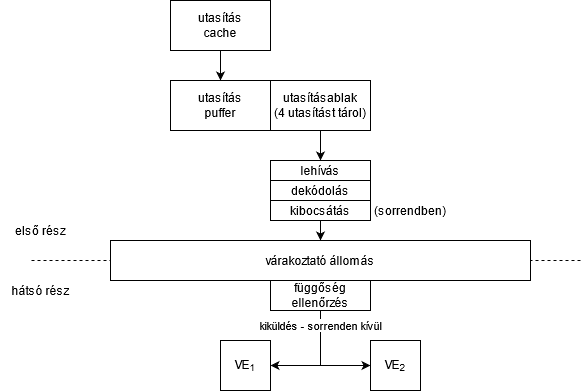
\includegraphics[width=0.8\textwidth]{kikuldes}
    \centering
    \caption{A sorrenden kívüli kiküldés működése RISC architektúrák esetén}
    \label{fig:kikuldes}
\end{figure}

\subsection{Regiszter átnevezés}
A dinamikus utasítás ütemezés ugyan növeli az átbocsátóképességet, viszont a függő utasításokat nem küszöböli ki, azok továbbra is lassítják a végrehajtást.
Erre jelent megoldást a regiszter átnevezés módszere, ami kiküszöböli az ál adatfüggőségeket.
Ez a WAR és WAW függőségeket küszöböli ki, azokat még kibocsátás előtt megszünteti (még mielőtt a várakoztató állomásba bekerül).
A függőség okát és a módszer leírását lásd részletesen: \ref{war}. és \ref{waw}. részek.
A gyakorlatban ennek eléréséhez a CPU minden regiszterhez rendel egy átnevezési (piszkozat) regisztert.
Ilyenkor az átnevezési logika követi az aktuális regiszter allokációkat, átnevezik a forrás regisztereket is, így az architekturális regisztereket elég csak a visszaíráskor figyelembe venni.
Az allokációt a CPU az utasításokhoz, és nem az architekturális regiszterekhez köti.
A forrás operandus megfelelő helyről való beolvasását a forrás regiszter átnevezés biztosítja.
Ha megszűnik a függőség, az utasítás végrehajtásra kerül és az eredmény visszaíródik az architekturális regiszterbe, majd az átnevezési regiszterek felszabadítása következik.
Ez a megoldás a dinamikus elágazásbecslés számára is előnyös, mivel ha kiderül, hogy a program mégse azon az ágon folytatódik, amihez az adott utasítást végrehajtottuk, az eredmény még csak a piszkozat regiszterben van jelen, ahonnan könnyen törölhető.

\subsection{Végrehajtási modell RISC architectúrák esetén}
A második generációs szuperskalár RISC architektúráknál az utasítások lehívása 128 bites buszon keresztül történik.
Ezután a processzor első részének feladata a dekódolás és az átnevezés.
A lehívás és a dekódolás általában 4 utasítás/ciklus szélesek.
A kibocsátás egy várakoztató állomásba történik (itt több tucat, ma már az x86\_64 architektúránál akár több száz utasítás is tárolódhat).
A függőség ellenőrzés itt, a várakoztató állomásban történik meg, ahonnan a végrehajtó egységek felé sorrendben kerülnek kiküldésre az utasítások.
Az operatív tár elérése a RISC architektúra miatt egy adat cache-en keresztül valósul meg, ami az architekturális regiszterekkel kétirányú kommunikációt folytat.
Az utasítások eredménye visszaírásnál az átnevezési regiszterekbe kerül, ahonnan ha minden rendben volt, visszaíródhat az architekturális regiszterekbe.
Az operandusok betöltése kétféleképpen történhet:
\begin{itemize}
    \item kibocsátáskor, vagy
    \item kiküldéskor.
\end{itemize}
Ha egy valós adatfüggőség miatt kibocsátáskor még nem áll rendelkezésre az operandus, az operandus helyére annak az átevezési regiszternek az azonosítója kerül, ahol majd a függőség feloldásához szükséges eredmény elő fog állni.
Az operandusok és a regiszter azonosítók megkülönböztetésére a CPU állapot biteket iktat a műveleti kódba az alábbi módon:
\begin{center}
    \begin{tabular}{ c | c | c | c | c | c | c }
        MK & OP\textsubscript{1} & A\textsubscript{1} & OP\textsubscript{2} & A\textsubscript{2} & OP\textsubscript{3} & A\textsubscript{3}
    \end{tabular}
\end{center}
Az állapot bitek értéke lehet 0, azaz operandus nem áll készen, vagy 1, ha az operandus készen áll.
0 értékű állapot bit esetén az utasítás a várakoztató állomásban van addig, amíg az operandus rendelkezésre nem áll.
Ekkor a kiküldés előtt az átnevezési regiszterből betöltődik az operandus, az állapot bit értéke pedig 1-re változik, az utasítás pedig végrehajtásra kerül.
\begin{figure}[h]
    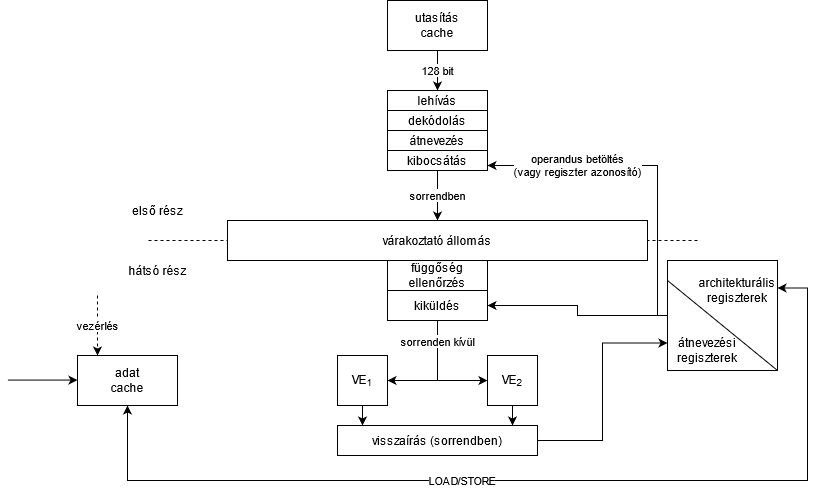
\includegraphics[width=\textwidth]{2gen_vegrehajtas}
    \centering
    \caption{A második generációs szuperskalár RISC architektúrák végrehajtási modellje}
    \label{fig:2gen_vegrehajtas}
\end{figure}

\subsection{Értékelés}
A második generációs szuperskalárok kibocsátási rátája kb. 3-4 utasítás/ciklus, a kiküldési ráta pedig általában 5-8 utasítás/ciklus.
Ezt nevezzük tölcsérszerű elvnek, azaz a processzor hátsó része felé haladva az átbocsátási képesség nő (szélesedik).
Ez a felépítés segít a szűk keresztmetszetek kiküszöbölésében.

\subsection{Kiküldéshez kötött operandusbetöltés}
A későbbi generációknál rájöttek a mérnökök, hogy fölösleges a kibocsátáskor betölteni az operandusokat.
Ezért úgy módosították az architektúrát, hogy a kibocsátásnál ugyan megmaradt a gépi kód struktúrája, de az állapot bitek minden esetben 0-ra voltak állítva, az operandusok helyére pedig a regiszter azonosító került.
A függőség ellenőrzés és az operandusok betöltése így mindig a kiküldés előtt történik, ami egyszerűsíti és gyorsítja a működést.

\subsection{CISC feldolgozás}
Újdonság, hogy a CISC utasításokat RISC-szerű utasításokká konvertálták.
Ez azért volt előnyös, mert a tapasztalat szerint a processzor általános felhasználás során az idő 80\%-ában az utasítások mindössze 20\%-át használja.
A CISC utasítások hossza általában 1-17 byte volt (Intel), ezeket konvertálták egységesen 128 bites, RISC-szerű utasításokká, amik aztán a fentebb látható módon kerültek végrehajtásra.
Az átalakítás a dekódolási fázisban, a RISC-CISC visszaalakítás pedig a visszaírás során történt.
Ez a felépítés (kívül CISC architektúra, belül RISC mag) máig jellemző az Intel processzorokra.
\paragraph{Utasítások aránya:} átlagosan egy CISC utasítás 1,2-1,5 RISC utasítássá konvertálható (az egyszerűbb CISC utasítások akár egy RISC-el is leírhatók, de a bonyolultabbakhoz akár 3-4 RISC utasítás is szükséges).
\paragraph{Kibocsátási ráta:} a konverzió miatt a CISC utasításokban mért kibocsátási ráta valamelyest csökken, nagyjából 3 utasítás/ciklusra.

\subsection{Függőségek kezelése}
Összefoglalva a második generációs szuperskalárok a következőképp kezelik a függőségeket:
\begin{itemize}
    \item Erőforrás függőség: több végrehajtó egység alkalmazása.
    \item Ál adatfüggőségek: regiszter átnevezés (100\%-os megoldás).
    \item Valós adatfüggőség: még mindig blokkol, részleges kezelés a várakoztató állomással, a sorrenden kívüli kiküldéssel és a spekulatív elágazáskezeléssel.
    \item Vezérlés függőség: spekulatív elágazáskezeléssel részleges kezelés.
\end{itemize}

\subsection{Utasítások végrehajtási sorrendje}
Egy utasítás akkor kerül kiküldésre a várakoztató állomásból, ha a bemenő operandusai rendelkezésre állnak $\rightarrow$ adatvezérelt (mohó/stréber) végrehajtási modell.

\subsection{Gyakorlati példa: Intel Pentium Pro}
\subsubsection{Tulajdonságai}
\begin{itemize}
    \item Kezdeti frekvencia: 133 MHz
    \item 14 fokozatú FX futószalag (nagy ugrást jelentett)
    \begin{itemize}
        \item hátrány: több függőség
        \item előny: a rövidebb fokozatok miatt növelhető a frekvencia
    \end{itemize}
    \item RISC-szerű utasításokat használ, ez is segített a rövidebb fokozatok elérésében.
    \item 20 bejegyzéses várakoztató állomás (vegyes, azaz egy helyen tárolta az FX, FP, stb. utasításokat)
    \item Szigorúan soros konzisztencia, ezt a ROB (ReOrder Buffer) biztosítja.
    \item A ROB végzi a regiszterátnevezést is.
    \item A lehívás 128 bites, itt fontos az utasítás határra illesztés (CISC miatt).
    \item A dekódolás során a CISC utasításokat RISC-be konvertálja, óraciklusonként 3 CISC utasítás hajt végre.
    \item A dekóder négy egységből áll, részei:
    \begin{itemize}
        \item D\textsubscript{1} - legfeljebb 4 RISC műveletté alakítható CISC utasítások dekódolása
        \item D\textsubscript{2} és D\textsubscript{3} - egy RISC műveletté alakítható CISC utasítások dekódolása (egyszerű dekódolók - összeadás, kivonás)
        \item MIS - 4-nél több RISC utasítássá alakítható utasítások dekódolása
    \end{itemize}
    \item A várakoztató állomás több független utasítás esetén mindig az idősebbet küldi ki végrehajtásra.
    \item A kívülről CISC architektúrának köszönhetően megmaradt a kompatibilitás, ugyanakkor a RISC mag miatt jelentősen javult a teljesítmény.
\end{itemize}

\subsubsection{Működése}
\begin{figure}[h]
    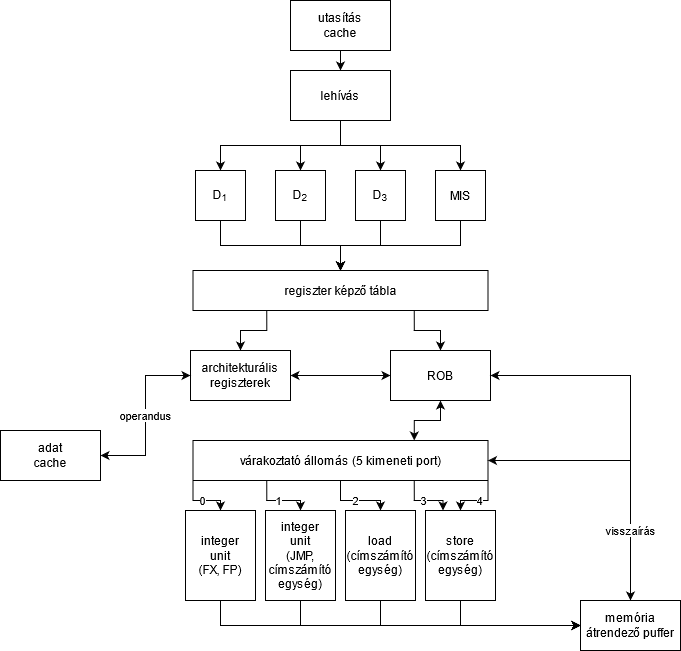
\includegraphics[width=\textwidth]{pentiumpro}
    \centering
    \caption{Az Intel Pentium Pro processzor működése}
    \label{fig:pentiumpro}
\end{figure}

\subsection{A reorder buffer működése}
A reorder bufffer tartalmazza az átnevezési regisztereket, vezérli a várakoztató állomást és a memória átrendező puffert.
A ROB-ot folyamatosan frissíteni kell a függőségek mielőbbi feloldása érdekében (tehát fontos, hogy az átnevezési regiszterazonosítók helyére bekerüljenek az operandusok).
Amikor egy eredmény előáll, a processzor asszociatív keresést végez (regiszterazonosító alapján), hogy a várakozó utasítások között van-e olyan, aminek operandusa a most előállt eredményt igényli.
Ha talál ilyet, az eredményt betölti a regiszterazonosító helyére és az állapot bitet 1-re állítja.
Ha mindkét forrás operandus állapot bite 1 lesz, a ROB kiküldi az utasítást a végrehajtó egységek felé.
\subsubsection{Szemléletése}
A működése egy kör alakú puffer segítségével ábrázolható (\ref{fig:rob}. ábra).
A várakoztató állomás a bemeneti és a végmutató között látható puffer regiszterekből áll.
Itt sorakoznak az i\textsubscript{n}-el jelölt utasítások.
Az utasítások a bemeneti mutatónál töltődnek be, a ROB elvégzi a regiszterátnevezéseket és beírja a forrás operandusokat, majd később az eredményt is az átnevezési regiszterekbe.
A bemeneti és végmutató között bármelyik független utasítás kiküldhető a végrehajtó egységek felé.
Ha egy utasítás végrehajtásra került, a bemeneti és a végmutató is egyel elmozdul, az ábrán az óramutatú járásával ellentétesen.
Ekkor már az i\textsubscript{x+n+1}-edik utasítás is része lesz a várakoztató tárnak.
\begin{figure}[h]
    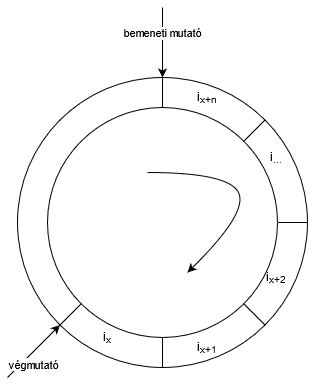
\includegraphics[width=0.4\textwidth]{rob}
    \centering
    \caption{A reorder buffer szemléltetése}
    \label{fig:rob}
\end{figure}
\subsubsection{Az utasítások sorrendisége}
Tegyük fel, hogy az ábrán látható utasítások közül i\textsubscript{x+1} és i\textsubscript{x+2} független utasítások és már megtörtént a végrehajtásuk, viszont i\textsubscript{x} függő utasítás és még nem történt meg a végrehajtása.
Ekkor az utasítások sorrendiségének biztosíítása érdekében i\textsubscript{x+1} és i\textsubscript{x+2} eredményei még nem írhatók ki a célregiszterekbe, azzal meg kell várniuk i\textsubscript{x} befejeződését, így a pufferregiszterek sem szabadulhatnak fel addig.
Ezzel látszólag i\textsubscript{x} végrehajtása ugyanúgy blokkoló hatású, viszont a teljesítmény mégis jelentősen növekszik, hiszen i\textsubscript{x} végrehajtásakor i\textsubscript{x+1} és i\textsubscript{x+2} eredményei már készen állnak, így csak ki kell írni őket.
Míg a végrehajtás akár 9-10 óraciklust is igénybe vehet, kiíráskor egy óraciklus alatt akár 5-6 utasítás eredménye is kiírható, ezáltal jelentős teljesítménynövekedést érünk el.
\subsubsection{Spekulatív bit}
A ROB minden utasításhoz rendel egy spekulatív bitet.
Azoknál az utasításoknál, amiknél még nem biztos a végrehajtás szükségessége (olyan elágazás részei, ahol a feltétel még nem került kiértékelésre), a spekulatív bit értékét 1-re állítja a ROB.
Amíg a spekulatív állapot fennáll, az eredmény nem írható ki, így biztosítva az utasítások sorrendiségét.
Ha az ugrási feltétel kiértékelésre került, két eset lehetséges.
Egyik, ha a kérdéses utasítást végre kell hajtani: ekkor a spekulatív bit 0-ra változik, az eredmény kiírásra kerül, a végmutató pedig elmozdul.
Mésik esetben, ha mégse kell végrehajtani az utasítást, az utasítás törlésre kerül a ROB-ból, az átnevezési (piszokzat) regiszter értéke felszabadításra kerül, a végmutató elmozdul, a helyes irányba történő utasítás pedig lehívásra kerül.
\subsubsection{Rekonverzió (RISC $\rightarrow$ CISC)}
Mivel egy CISC utasítás több RISC utasítássá konvertálódik a végrehajtásra, de a rendszer kívülről CISC architektúrájú, az egy CISC utasításhoz tartozó RISC utasítások eredményei csak akkor írhatók ki, ha már mindegyiknek előállt az eredménye.
Így az eredmények egyszerre kerülnek kiírásra és megtörténhet a rekonverzió.

\section{Harmadik generációs szuperskalárok}
A második generációs szuperskalárok a fent említett módszerekkel elérték az architektúra teljesítménybeli korlátait, így más irányba kellett fejleszteni.
Így jelent meg 1997 környékén az utasítás szintű párhuzamosság, amivel elérkeztek a harmadik generációs szuperskalár CPU-k.
Egyesek szerint nincs haramadik generáció, hanem ez csak a második generáció kibővítése multimédiás/3D képességekkel.

\subsection{Utasításon belüli párhuzamosság típusai}
\begin{itemize}
    \item Duál műveleti utasítások (pl. multiply-add: $y=ax+b$. Elsősorban numerikus feldolgozást segíti, általános alkalmazásoknál ritka).
    \item SIMD utasítások (Single Instruction Multiple Datastream - több operanduson ugyanazon utasítás elvégzése. Ilyen pl. az Intel MMX PADDW utasítása, ami 4 fixpontos összeadást végez el egy utasítás alatt).
    \item VLIW architektúrák
\end{itemize}

\subsection{SIMD jellemzői}
\begin{itemize}
    \item A SIMD utasítások egy kibővített utasításkészletet alkotnak (multimédiás utasításokkal).
    \item A logikai architektúra kibővítését igényli.
    \item 8 bemenő operandus szükséges $\rightarrow$ sokszorosára nő a memóriaigény.
    \item A növekvő memória sávszélesség miatt az L2 cache közös lapkára kerül a CPU-val (ez korábban, pl. a Pentium II-nél külön foglalatba került, ez volt a slot 1).
    \item A gyorsabb megjelenítés érdekében a buszrendszer is bővült (pl. AGP - Advanced Graphics Port, PCI express).
    \item 3D alkalmazásokat, játékokat tett lehetővé.
    \item Először az Intel Pentium processzorban (1997) jelent meg MMX (MultiMedia eXtensions) néven, ami egyelőre csak fixpontos multimédiás utasításokat támogatott.
    \item Az MMX technológia kibővítésre került a Pentium III processzorban (1999), SSE (Streaming SIMD Extensions) néven, ami már lebegőpontos utasításokat is tartalmazott.
    \item A processzor általános teljesítménye nem nőtt jelentősen a SIMD bevezetésével, viszont a multimédiás alkalmazásokat (kép, videó, 3D játék) jelentősen meggyorsította, mivel ezeknél nagy mennyiségű, függőség nélküli adattal kell dolgozni.
\end{itemize}

\subsection{Fixpontos SIMD feldolgozás}
A fixpontos SIMD utasítások elsősorban a hang, és a pixeles megjelenítést használó multimédiás alkalmazásokat gyorsítják.
Egy utasításban 2-8 operandus lehetséges.
(A lebegőpontos SIMD utasítások a vektoros és 3D alkalmazásokat gyorsítják, utasításonként 2-4 operandussal rendelkeznek.)
\subsubsection{Hangfeldolgozás}
A hangot a feldolgozásához először digitalizálni kell.
Ezt az analóg jelből történő, meghatározott időközönkénti mintavételezéssel érhetjük el.
Ebben a formában már tárolható és visszajátszható.
A minőséget befolyásolja a mintavételezés sűrűsége (felbontás), ennek növelése jobb minőséget, de nagyobb erőforrásigényt jelent.
Példa: 50 kHZ-es mintavételezés $\rightarrow$ 50 ezer minta másodpercenként (kb. DVD minőség).
A hangfeldolgozás másik jellemzője, hogy egy adott mintát hány biten tárolunk (minta nagysága).
8 bit esetén 256 féle hangmagasságot tudunk tárolni.
A cél, hogy minnél jobban hasonlítson a digitális jel az eredeti, analóg függvényhez.
\subsubsection{Hang tömörítése}
Ebben az időben még nem állt rendelkezésre annyi tároló kapacitás, hogy jó minőségű jeleket lehessen tárolni, ezért született meg a tömörítés.
A különböző tömörítési formátumok (AVI, MP3) használatával nagyrészt minőség romlás nélkül tudták csökkenteni az adatok mennyiségét.
A SIMD utasítások segítségével ezeket a tömörített formátumokat valós időben lehet lejátszani.
\subsubsection{Képfeldolgozás}
A képek esetén képpontokat tárolunk el, minden képponthoz hozzá kell rendelni a színét és a fényességét.
A színek három értékből állnak össze: piros, zöld és kék.
A színek előállításához használjuk a színfordítási táblázatot, amiben minden színhez egy számérték van hozzárendelve.
Ez alapján áll elő a színskála kódolása.
Kezdetben 1 biten tárolták az értékeket (világos/sötét), aztán a színes kijelzők megjelenésével ez 8, később 16 (hicolor), végül 24 (truecolor) bitre bővült.
A 32 bites színskálán 24 biten ábrázolják a színeket, a többi 8 bit pedig az alfa csatorna, ami az effekteket tárolja (pl. átlátszósági mutató).
\subsubsection{Probléma}
A hang és kép feldolgozása során tehát a problémát a nagy mennyiségű adat tárolása és feldolgozása okozza.
\subsubsection{Megoldás}
\begin{itemize}
    \item Kezdetben célhardverrel, multimédiás kártyákkal.
    \item Később a CPU multimédiás bővítésével.
\end{itemize}
\subsubsection{Bit-blokk átvitel és pakolt adattípusok}
A multimédiás megjelenítés tipikus művelete a bit-blokk átvitel.
Lényege, hogy minden megnyitott ablakot egy bit-blokkként kezelünk, így nem egyesével dolgozunk az operandusokkal.
Ez szükséges, mivel például egy 1920x1080-as kijelző 24 bites színskála esetén kb. 6 MB adatot jelent, ami azt jelenti, hogy 30 FPS megjelenítés esetén 180 MB/sec feldolgozási sebességre lenne szükség.
Ez a sebesség még ma is soknak számít, ezért a megoldására egyrészt tömörítést alkalmaztak, másrészt pedig architekturális megoldást vezettek be.
Az architekturális megoldás egy új fixpontos adattípus bevezetése, a pakolt adattípus.
A pakolt adattípus az Intel MMX processzorokban jelent meg először, típusai:
\begin{itemize}
    \item pakolt byte (8 bit hossz * 8 db = 64 bit)
    \item pakolt félszó (16 bit hossz * 4 db = 64 bit)
    \item pakolt szó (32 bit hossz * 2 db = 64 bit)
\end{itemize}
A SIMD utasításoknak köszönhetően ezeket az adattípusokat egy utasítás alatt össze tudták adni az Intel MMX CPU-k.
Ezek az új utasítások a következőek:
\begin{itemize}
    \item 4 alapművelet
    \item logikai műveletek mindhárom pakolt adattípusra
\end{itemize}
A multimédiás alkalmazások nagyrészt az internet elterjedése miatt lettek szükségesek.
\subsubsection{Fizikai architektúra}
A pakolt adattípusok feldolgozásához az architektúra fizikai módosítására is szükség volt:
\begin{itemize}
    \item 64 bites regiszterek (új regiszterek helyett a lebegőpontos regiszterek használata, amik 80 bitesek voltak, így megfeleltek a 64 bit tárolására)
    \item 64 bites buszrendszer (először belső, majd külső buszok is)
    \item Pentium II-es processzorban már két MMX futószalag került beépítésre, ami tényleges gyorsítást jelentett a függőségek hiánya miatt
\end{itemize}

\subsection{Lebegőpontos SIMD feldolgozás}
A lebegőpontos SIMD utasítások a vektoros képfeldolgozást segítik, aminek használatával a feldolgozandó adat mennyisége csökkenthető.
\subsubsection{Vektoros képfeldolgozás}
Egyenesekkel vagy görbékkel határolt obejktumok geometriai jellemzőkkel leírhatók.
Példa: egy egyenes ábrázolása Full HD kijelzőn keresztben 1920 képpontot jelent fixpontosan, ennyi adatot is kell tárolnunk.
Vektorosan azonban elég a két végpontot eltárolni, ami lényegesen kevesebb adatot jelent.
Kör esetében elégséges a középpont és a sugár tárolása.
A módszer eredménye, hogy jóval kevesebb adatot kell tárolnunk, viszont a megjelenítéshez sokkal többet kell számolni.
Képek tárolása is lehetséges így, ha azokat geometriai alakzatokra bontjuk fel, majd ezeknek az adatait tároljuk.
Az első 3D játékok is ilyen elven működtek.
Előnye, hogy a képek könnyen mozgathatók, kicsinyíthetők és nagyíthatók.
A lebegőpontos ábrázolás szükséges, mivel a geometriai műveletek során törtekkel is kell számolni.
Hátránya, hogy 2D ábrázolásnál az éles határok miatt kevésbé hasonlít a valóságra, ennek kiküszöbölésére textúrákat alkalmaznak.
\subsubsection{3 dimenziós ábrázolás}
3D ábrázolásnál értelmezni kell egy harmadik dimenziót a 2D-s képen.
Az élethű megjelenítéshez biztosítani kell, hogy a párhuzamosok a végtelenben összetartanak, hogy a közelebbi obejktumok nagyobbnak hassanak, valamint az atmoszférikus hatást (a távolabbi obejktumok halványabbak és kékesebbek).
A 3D-s filmeknél minimum 15-30 FPS-t kell előállítani.
Ehhez kb. 500 000 objektum megjelenítése szükséges másodpercenként $\rightarrow$ nagy mennyiségű lebegőpontos adat feldolgozására van szükség.
\subsubsection{Példa - az Intel Pentium III}
Ilyen lebegőpontos feldolgozásra először az Intel Pentium III-as processzora volt képes, az SSE kiterjesztéssel.
A CPU 500 MHz-en működött és nagyjából 2 GFLOPS/sec számítási kapacitással bírt.
Ez azt jelenti, hogy másodpercenként 2 milliárd lebegőpontos műveletet tudott végrehajtani.
A mai processzorok kb. 12-20 GFLOPS/sec teljesítményt biztosítanak.
\subsubsection{Logikai architektúra}
Logikai oldalról nézve mindez egy új utasításkészletet jelentett, ez az SSE (ld. feljebb).
Kb. 70 db új utasítást tartalmazott, amik a lebegőpontos pakolt adattípusokkal tudtak műveleteket végezni.
Az adatok 128 bites pakolt típusok voltak:
\begin{itemize}
    \item 4 * 32 bit - egyszeres pontosság, vagy
    \item 2 * 64 bit - kétszeres pontosság.
\end{itemize}
Ezek megfelelnek az IEEE 754-es szabványnak, ami a lebegőpontos számokra vonatkozik.
\subsubsection{Fizikai architektúra}
Itt már szükség volt ténylegesen új regiszterek létrehozására, így 8 db új 128 bites regiszter került a processzorokba.
Ezek mentéséről és töltéséről az operációs rendszer vagy az adott szoftver gondoskodik.
Az első szoftveres támogatás a Windows 98-ban jelent meg.
Az új regiszterek bevezetésével 1985 óta először változtatta meg az Intel a processzorok regiszterkészletét.
Következménye, hogy a megszakítás rendszert is át kellett tervezni, és ez az OS gyártójával való együttműködést igényelte.